\chapter{State of the Art}
\label{cha:StateOfTheArt}

To answer the posed questions (see chapter \ref{cha:Introduction}), the attention during research was directed to pose estimation of articulated objects. A majority of the selected reference papers focus on the pose extraction of a human body. Depending on the approach different steps are required which can be generally subdivided into the digitalization of the object to be captured (see subsection \ref{sec:reconstruction}) and its segmentation into rigid parts (see subsection \ref{sec:segmentation}). Regardless of the chosen approach many difficulties have to be overcome in order to estimate the joints and skeleton. A key role of the pose estimation method constitutes the registration of surfaces (see section \ref{registration}). It is commonly referred to as an optimization problem as the goal is to detect the best possible outcome.
%
\begin{figure}[H]
	\centering
	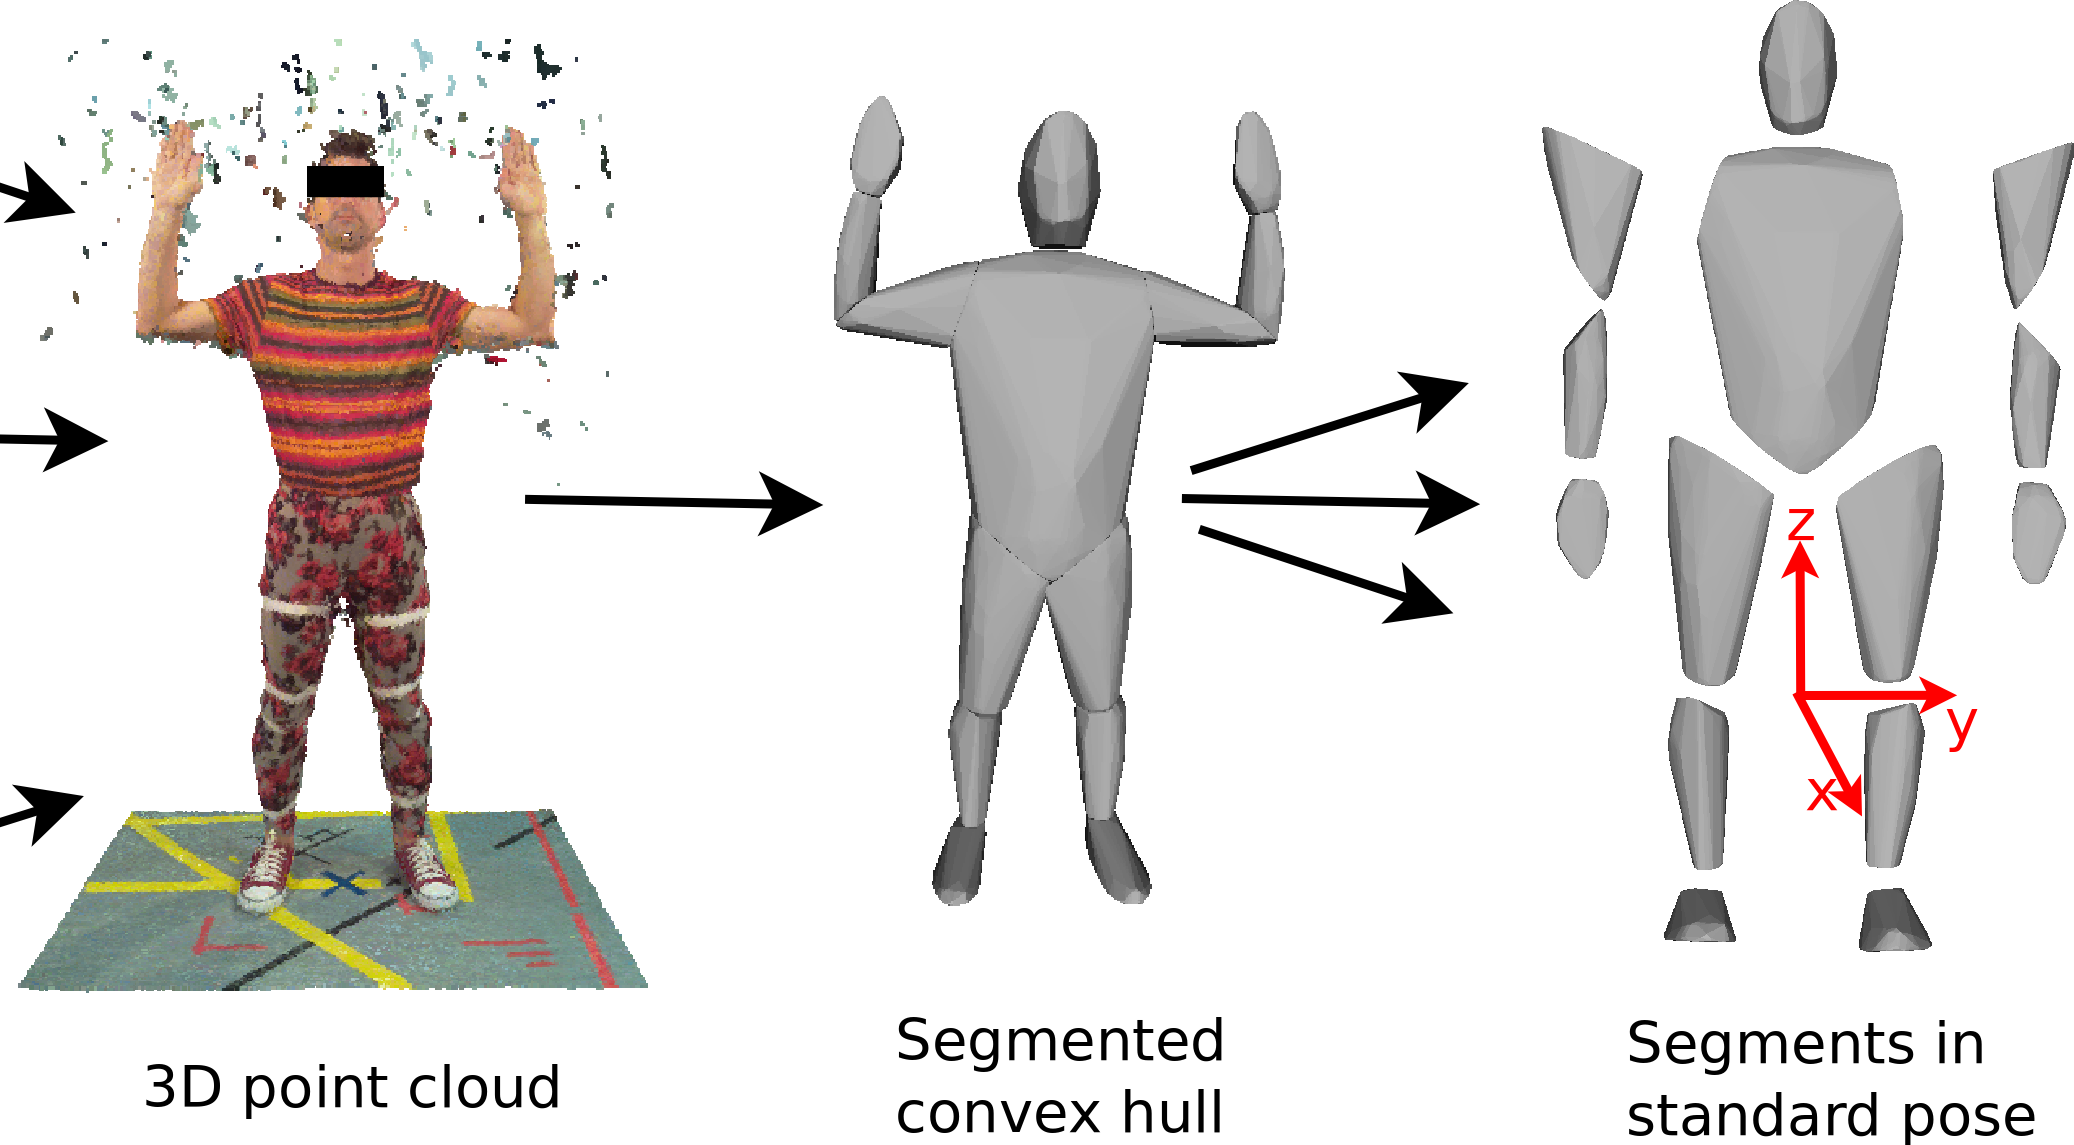
\includegraphics[width=0.7\linewidth]{reconstructionWorkflow}
	\caption{General pose estimation approach. As a first step the captured object needs to be digitalized (a) and if required reconstructed(b) to a mesh. Then, it needs to be segemented into its rigid parts (c) which is the key part in order to estimate the joints and skeleton.}
	\label{fig:posecapture}
\end{figure}
%
%TODO: new image with puppet! --> picture, point cloud, skeleton
%
\section{Registration}
\label{registration}
Generally, registration in computer vision and computer graphics refers to the alignment of overlapping components of two or more digital data sets \cite{survey}. Thereby, the most essential part is the detection of point correspondences between two surfaces to be registered often supported by RANSAC \cite{ransac}. One main application is the alignment of two or more incomplete range scans of an object from different view ports to obtain a complete model. Further applications are symmetry detection, articulation of non-rigid objects and subpart identification. For this reason a vast number of pose estimation and skeleton extraction approaches rely on a successful registration. A discriminated between rigid and non-rigid registration can be done. In the former case, it is assumed that two surfaces are related by a rigid transformation which can seen on figure \ref{fig:registration}~(a). A well-known approach for a rigid registration is the iterative closest point (ICP) \cite{ICP}. It requires a similar initial position of two shapes to avoid a local optimum. For this purpose it is often taken advantage of the principal component analysis (PCA) of shapes. With each iteration step the point correspondences between two input objects are updated by selecting the closest points. As a next step, the rigid transformation between two shapes is recalculated considering the detected correspondences. A matching error $e$ is achieved, which states the total euclidean distance between the associated points of the registered shapes. The algorithm terminates after a predefined number of iterations or if a specified value for $e$ is achieved. Considering two non-rigid surfaces composed of rigid parts (e.g. a human), the rigid registration will not lead to a convincing result as the individual rigid parts may undergo varying rigid transformations. In this case a non-rigid registration is required, which performs a segmentation into rigid parts which can be seen on figure \ref{fig:registration}~(b).
%
\begin{figure}[H]
	\centering\small
	\begin{tabular}{cc}
		\fbox{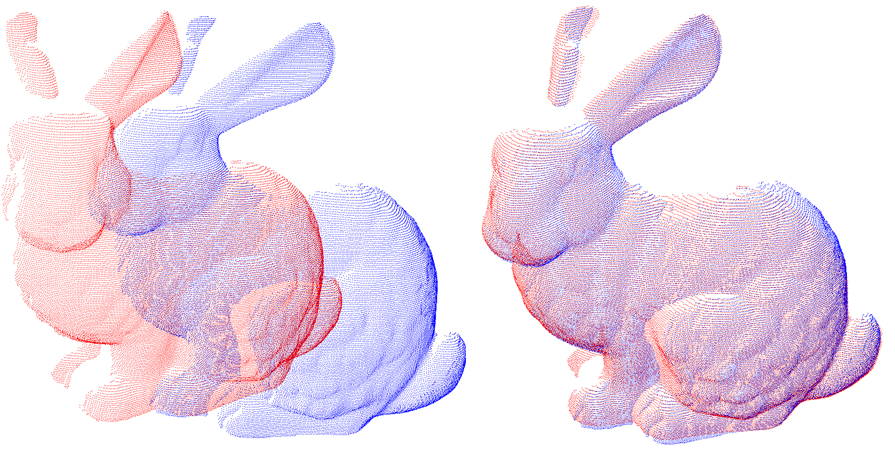
\includegraphics[width=0.43\textwidth]{stanfordBunny}} &		% JPEG file
		\fbox{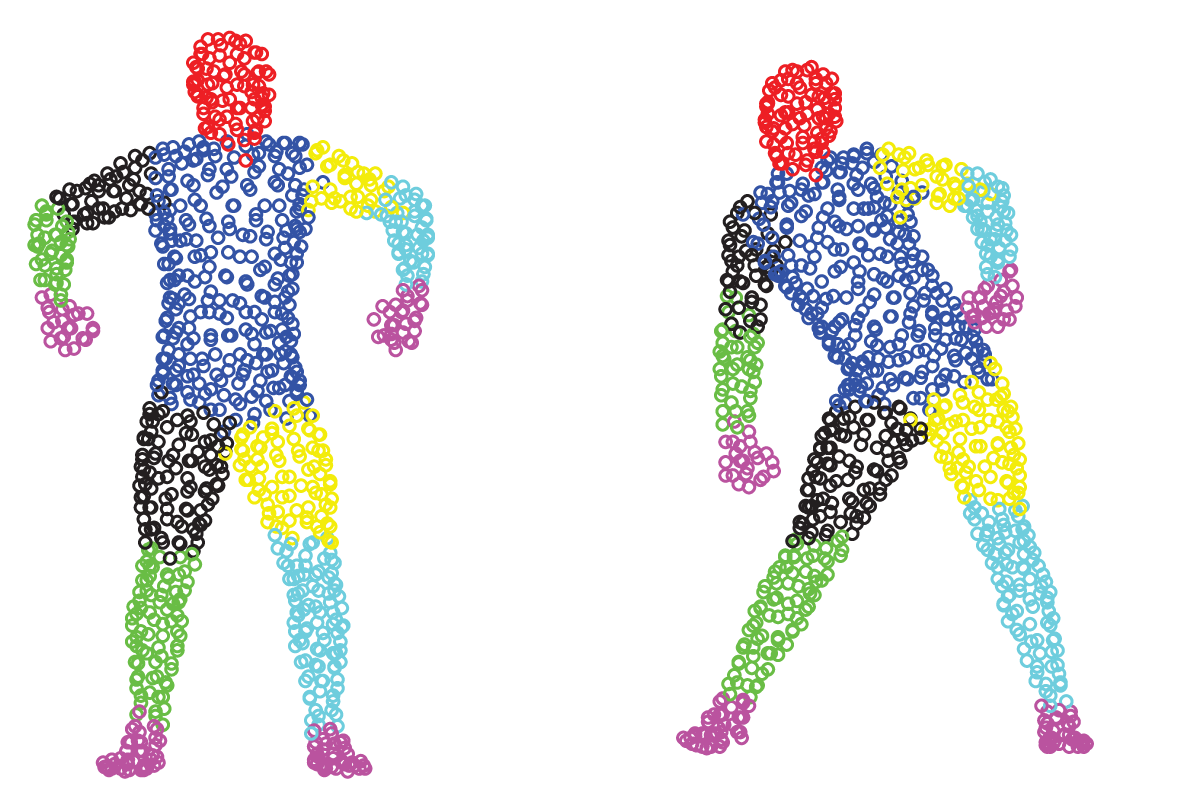
\includegraphics[width=0.45\textwidth]{nonrigidregistration}} 
		\\	% PNG file
		(a) & (b) 
	\end{tabular}
	\caption{Rigid registration of a rigid model of the stanford bunny~(a) \cite{stanfordBunny} and non-rigid registration of a human~(b) \cite{registrationHuman} composed of several rigid parts.}
	\label{fig:registration}
\end{figure}\textbf{}
%
Some factors complicate the accomplishment of a visual successful registration. Main difficulties are noisy data and outliers which often arise from low resolution scans. Furthermore, there might only be a limited number of overlapping data which is the case for multiple incomplete scans of an object from different view ports. Self occlusion and variations form initial poses are influence factors which should not be underestimated. In case of non-rigid registration the main difficulty is the establishment of correspondences as several transformations of the data need to be considered.
%
\section{Pose estimation of articulated objects}

To successfully estimate the pose of an articulated object, generally two main parts have to be performed: the digitalization of the object and the segmentation of the data into rigid parts. As this thesis focuses on the segmentation of the input data into rigid parts, the digitalization of the object will not be covered in detail. 

\subsection{Digitalization of the object}
\label{sec:reconstruction}
As a first step the object to be captured needs to be digitalized for the subsequent segmentation step. By a scanning step the real shape is collected as 2D or 3D data. The raw data in form of 2D images, video streams, or even point clouds in 2D or 3D can be directly used for pose estimation. Multiple commercial 3D scanner are available strongly varying in precision and resolution and purchase price. Especially, RGB-D sensors (Kinect) have taken on greater significance for 3D reconstruction !!!REF KINECT!!! as they are easily accessible and inexpensive. Usually, a subsequent reconstruction step is performed which converts the raw data into a mesh often combined with registration of different scans. Reconstruction from images and videos gets more and more popular as they are independent from expensive scanner. !!!REF
Voxelization, Shape from Silhouette, Shape from Shading, 2d images!!! Some approaches also skip the digitalization step and take a 3D mesh as input from a modeling software. Shape from silhouette \cite{mocap}
%
%TODO: add scanning/reconstruction methods
%
\subsection{Segmentation}
\label{sec:segmentation}

The crucial computer vision part of the pose estimation is the segmentation of the digitalized object into its rigid parts in order to estimate joints and the skeleton. The main idea is to allocate each data point of an input object to a rigid part. For that, additionally to the input data any kind of prior information is indispensable. Regarding the non-rigid registration the same object in another configuration is required which is usually referred to as a \textit{template}. To generally reduce the correspondence space specific constraints can be set. Those classify the different segmentation approaches into supervised (see section \ref{supervised}) and unsupervised methods (see section \ref{unsupervised}) whereby the former depends on user input before the segmentation algorithm. 

\section{Supervised methods}
\label{supervised}

Supervised methods for pose estimation greatly simplify the segmentation procedure as certain assumptions of the object can be made. Examples include the placement of markers on the real object or the digitalized model to have prior information of its joints linking the rigid parts !ADDREFERENCES!. Furthermore, the usage of an \textit{object model} is considerable used to have prior knowledge of the number of rigid parts and possibly the length and shape of an object (see \cite{multiLayerSkeleton}, \cite{de2008hierarchical} and \cite{michoud2007real}). Another well known approach is to use the motion information of known point correspondences from sequences (see \cite{segmentationMotion}, \cite{animatedObjects}). The approach from \cite{sfsMocap} sequentially estimates each joint by the person being captured moving one body part at a time. By extracting and registering the resulting CSPs (colored surface points) a joint can be estimated which can be seen on figure \ref{fig:supervisedMotion}.

%TODO: add picture of csp

\begin{figure}[H]
	\centering
	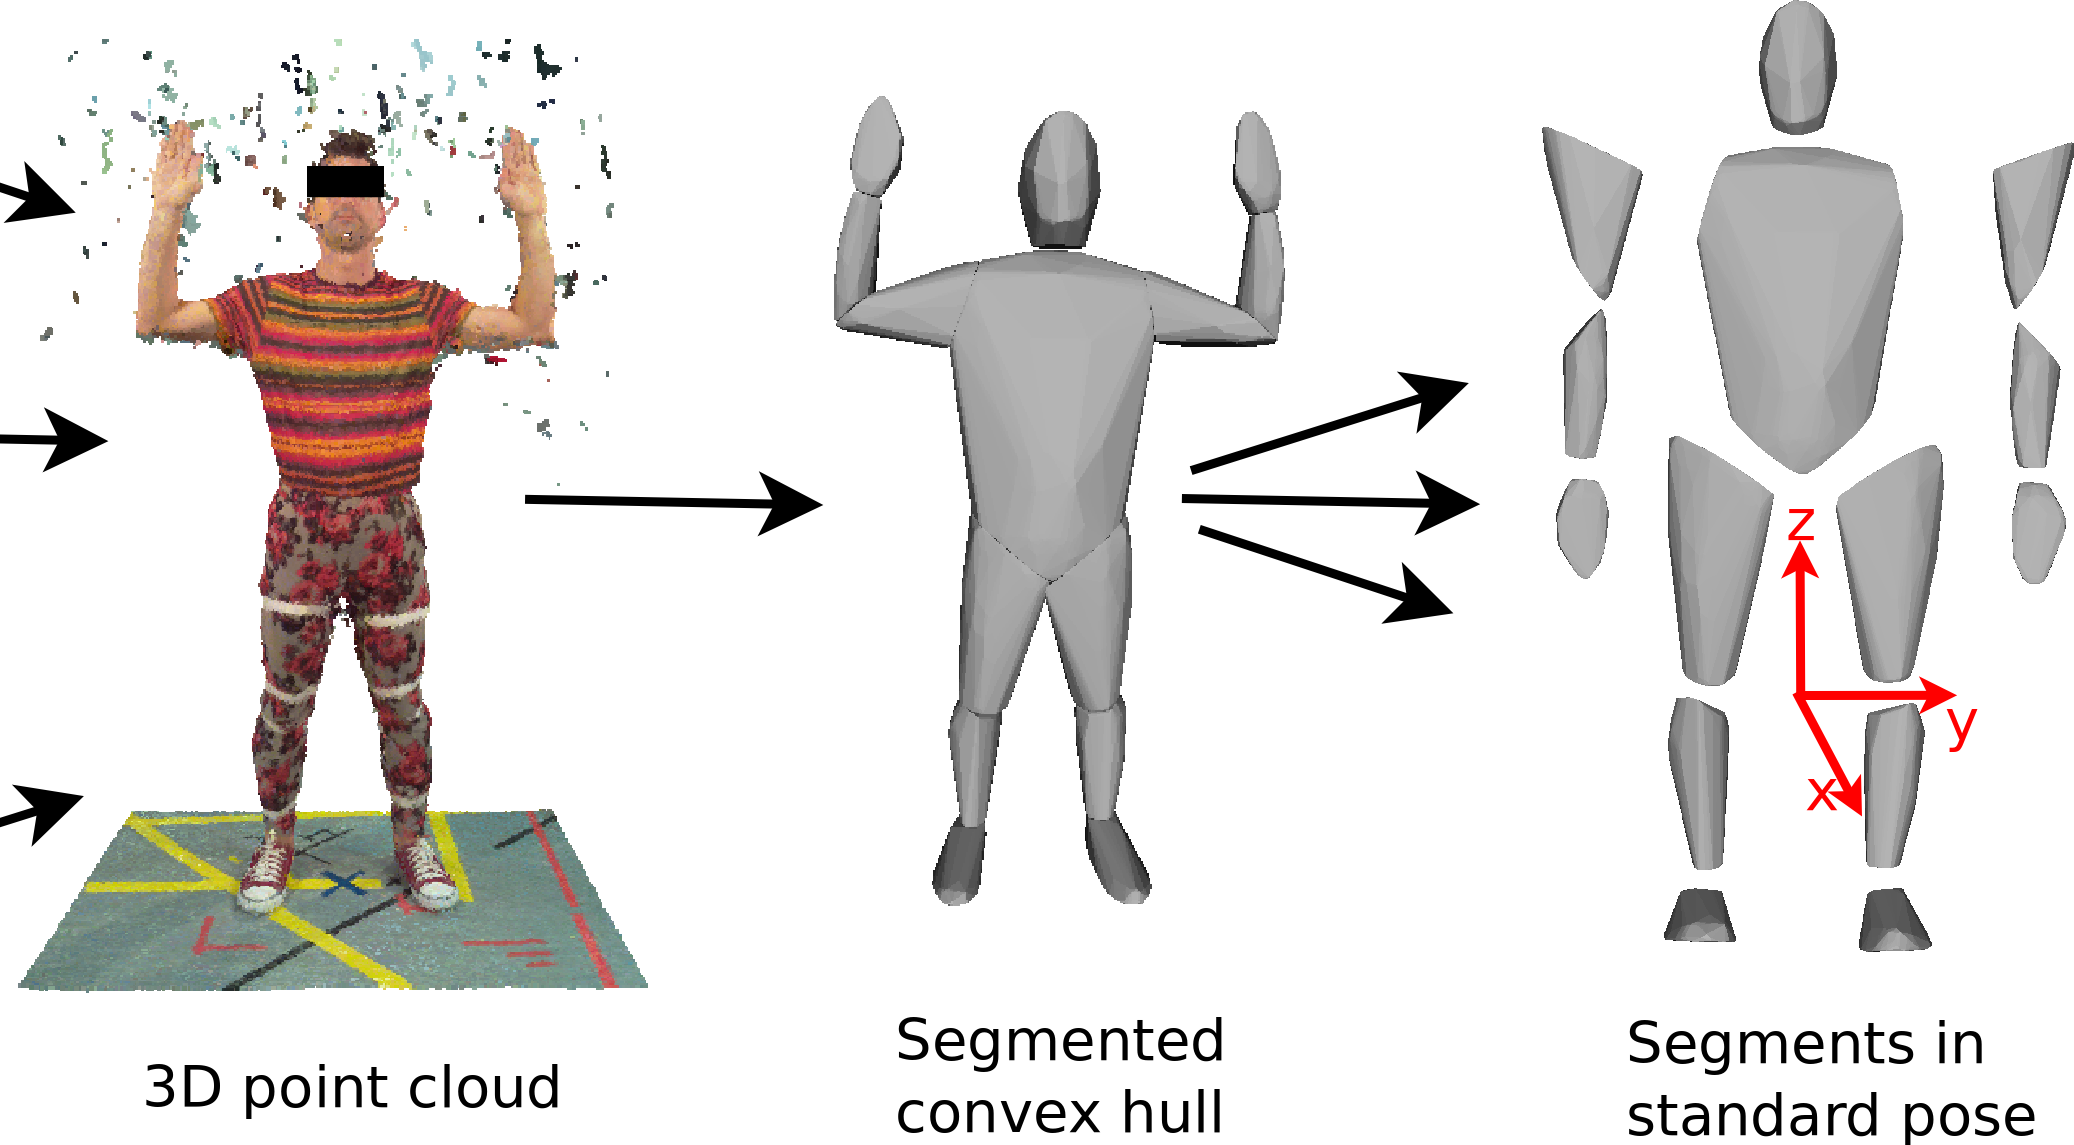
\includegraphics[width=0.7\linewidth]{reconstructionWorkflow}
	\caption{General pose estimation approach. As a first step the captured object needs to be digitalized (a) and if required reconstructed(b) to a mesh. Then, it needs to be segemented into its rigid parts (c) which is the key part in order to estimate the joints and skeleton.}
	\label{fig:supervisedMotion}
\end{figure}


\section{Unsupervised methods}
\label{unsupervised}

Although the approaches mentioned in section \ref{sec:currentApproaches} work quite well depending on the application, improvements can be made that are more independent from user inputs. For example the computation of features, ... which leads us to the non-rigid registration \ref{nonrigidregistration}.

\subsection{Challenges}
\label{Challenges}
There are many challenges regarding the non-rigid registration of point clouds in 2D, as well as in 3D. First off, the input data can be noisy by means of points not belonging to the object. Furthermore, the approach is computationally expensive and time-consuming, as the corresponding body parts of two meshes need to be detected iteratively. Additionally, the inevitable difficulty of finding the global optimum, related to ambiguous body parts, has to be overcome.

\subsection{Related work}
\label{sec:RelatedWork}

By focusing on approaches computing the segmentation of articulated objects from 3D data, many different ones could be detected. They face similar challenges (see subsection \ref{Challenges}) but solve them in different ways
%%
\subsection{Correlated Correspondence}

A main approach for non-rigid registration is proposed by Anguelov \cite{Anguelov04} applying the correlated correspondence algorithm \cite{CorrelatedCorrespondance}. The algorithm takes a \textit{template} Mesh $D_0$ and other Meshes $D_1,\ldots,D_n$ in different configurations as input. The algorithm then performs a probabilistic framework and Expectation-Maximization (EM) to iterate between finding a decomposition of the \textit{template} into rigid parts and detecting them in the other meshes. Furthermore, a random clustering is applied to facilitate the detection of associated rigid parts.
%%
%TODO: images?
%%
A different approach proposes the recursive detection of body parts by the LRP -- ``largest rigid part'' algorithm \cite {guo2016correspondence}. 
%%
\subsection{LRP}
The LRP algorithm discovers the articulated parts of two objects in different configurations by initially detecting the largest rigid part. This would be the biggest point cluster by applying a single rigid transformation. To reach that, sparse correspondences in combination with RANSAC are implemented. From there, the linking parts are recursively detected by growing clusters from the LRP and reapplying the algorithm. 
%%
%TODO: images?
%%
Another approach is achieved by Symmetrization \cite{Mitra07}, by detecting and aligning the body parts’ symmetry axes of an object(see figure \ref{fig:Symmetrization}). Based on Anguelov \cite{Anguelov04} and Mitra \cite{Mitra07}, Chang et al developed a closely related approach \cite{chang08articulated} \cite{chang09range}.
%%
%TODO: images?
%%

%TODO: Add other references
\subsection{Possible improvements}

%TODO: What are the main deficits of the algorithms?

The proposed approaches achieve convincing results concerning the accuracy of the segmentation and the detection of rigid parts. However, they are all computationally expensive and require a considerable number of computation steps to iteratively detect rigid parts in two associated objects. This reflects on the run time of the algorithm which offers therefore great potential for improvements.

Taking the existing methods as reference (see chapter \ref{cha:RelatedWork}) a new segmentation approach is developed. Thereby, the main focus is to reduce the computation steps of the correlated correspondence algorithm \cite{CorrelatedCorrespondance} as well as the LRP algorithm \cite {guo2016correspondence}. To fully focus on the segmentation into its rigid part, the 3D reconstruction of the articulated object is assumed to be available.